\documentclass[12pt]{ctexart}
\usepackage{amsmath}
\usepackage{graphicx}
\usepackage[hmargin=1.25in,vmargin=1in]{geometry}
\usepackage{subfig}
\usepackage[colorlinks=true,bookmarks=true,bookmarksnumbered=true]{hyperref}

\title{声光效应 实验报告}
\author{71120226 陈宇轩}
\date{2021 年 11 月 1 日}

\begin{document}
    \maketitle

    \section{实验目的}

    \begin{itemize}
        \item 了解声光效应的原理;
        \item 了解布拉格衍射的实验条件和特点;
        \item 利用布拉格衍射计算介质中声波的速度。
    \end{itemize}

    \section{实验原理}

    超声波在介质中传播时,会引起介质的弹性应变作时间和空间上的周期变化,并令介质的折射率也作
    相应的变化。光通过这个介质时,就会发生衍射,如同经过相位光栅一般。这就是声光效应。

    发生布拉格衍射时,介质中声波的速度 $v_s$ 与光的偏转角 $\Phi$ 以及声波的频率 $f_s$
    有以下关系:

    \begin{equation}
        \Phi \approx \frac{\lambda}{\lambda_s} = \frac{\lambda_0}{v_s}f_s
    \end{equation}

    已知 $\lambda_0 = 650\mathrm{nm}$,通过测算出 $\Phi$,$f_s$ 的值,即可
    计算出 $v_s$ 的值。

    实验中,由于 $\Phi$ 较小,可以用 $\frac{\Delta L}{L}$ 来近似代替,其中 $\Delta L$
    是光经过介质后到光强仪的偏转距离,$L$ 是介质到光强仪的距离。

    \section{实验仪器}

    见表 \ref{components}。

    \begin{table}[hp]
        \centering
        \caption{声光效应 实验仪器表}
        \label{components}
        \begin{tabular}{|c|c|c|}
            \hline
            仪器名称 & 型号 & 生产厂家 \\ \hline
            CCD 光强分布测量仪 & LM601S & 南京浪博科教仪器有限公司 \\ \hline
            声光效应功率信号源 & SO-2000 & 南京浪博科教仪器有限公司 \\ \hline
            示波器 & YB43020B & 江苏绿扬电子仪器集团有限公司 \\ \hline
        \end{tabular}
    \end{table}

    \section{实验过程}

    \begin{enumerate}
        \item 调节实验仪器;
        \item 观察声光效应的现象:光经过介质后在屏上产生衍射纹,如图 \ref{sp02} 所示,除非介质中没有施加声波;
        \item 撤去屏,令衍射纹射入 CCD 的光敏面;
        \item 确认示波器中 0 级光所对应的条纹,并尝试定格;
        \item 调整元件偏转角,令示波器中 1 级光光强大于 0 级光,以后保持光学元件不动;
        \item 不断调整声波频率,每次调整完成后记录新的 $\Delta L$ 和 $f_s$ 值;
        \item 计算。
    \end{enumerate}

    \section{数据记录}

    见表 \ref{result}。

    \begin{table}[hp]
        \centering
        \caption{声光效应 实验数据记录表}
        \label{result}
        \begin{tabular}{|c|c|c|c|}
            \multicolumn{4}{r}{\small{L = 504.5mm}} \\ \hline
            $\Delta L$/mm & $\Phi (\times 10^{-2})$ & $f_s$/MHz & $v_s$/$\mathrm{m} \cdot \mathrm{s}^{-1}$ \\ \hline
            6.138 & 1.218 & 80.09 & 4274 \\ \hline
            6.534 & 1.295 & 84.99 & 4266 \\ \hline
            6.798 & 1.347 & 90.00 & 4343 \\ \hline
            7.194 & 1.426 & 95.01 & 4331 \\ \hline
            7.590 & 1.504 & 100.00 & 4322 \\ \hline
            7.986 & 1.583 & 104.02 & 4320 \\ \hline
            8.316 & 1.648 & 110.04 & 4354 \\ \hline
            8.646 & 1.714 & 114.99 & 4361 \\ \hline
            9.306 & 1.845 & 120.00 & 4216 \\ \hline
            \multicolumn{1}{|c}{平均值} & \multicolumn{2}{c}{} & \multicolumn{1}{c|}{4310} \\ \hline
        \end{tabular}
    \end{table}

    根据表 \ref{result} 的数据得出结论:超声波在目标介质中的传播速度为 $4310 \mathrm{m} \cdot \mathrm{s}^{-1}$。

    \section{实验结论}

    \begin{itemize}
        \item 超声波在目标介质中的传播速度为 $4310 \mathrm{m} \cdot \mathrm{s}^{-1}$;
        \item 实验中确实观察到了当超声波存在时屏上出现了衍射纹,且关闭超声波发生装置后衍射纹消失,验证了声光效应;
        \item 一般 0 级光不会因为声波的改变而改变;发生布拉格衍射时,通常会有次级光比 0 级光强;
        \item 存在一定声波频率,在该频率后,无论如何偏转介质与声波,1 级光都不会强于 0 级光(本实验中该频率为 120 Hz);
        \item 在定格时,示波器上波形每 2 个周期之间的低谷是由于传感器延迟所致,在定格时注意波形周期的起点为上升沿 80\% 处,终点为下降沿 20\% 处。
    \end{itemize}

    \section{附件}

    \begin{figure}[hp]
        \centering
        \caption{观察声光现象在屏幕上的衍射纹}
        \label{sp02}
        {\small 光束在穿过加有声波的介质后在屏上产生了明显的衍射纹,停止附加声波后衍射纹消失。此处仅展示衍射纹。}
        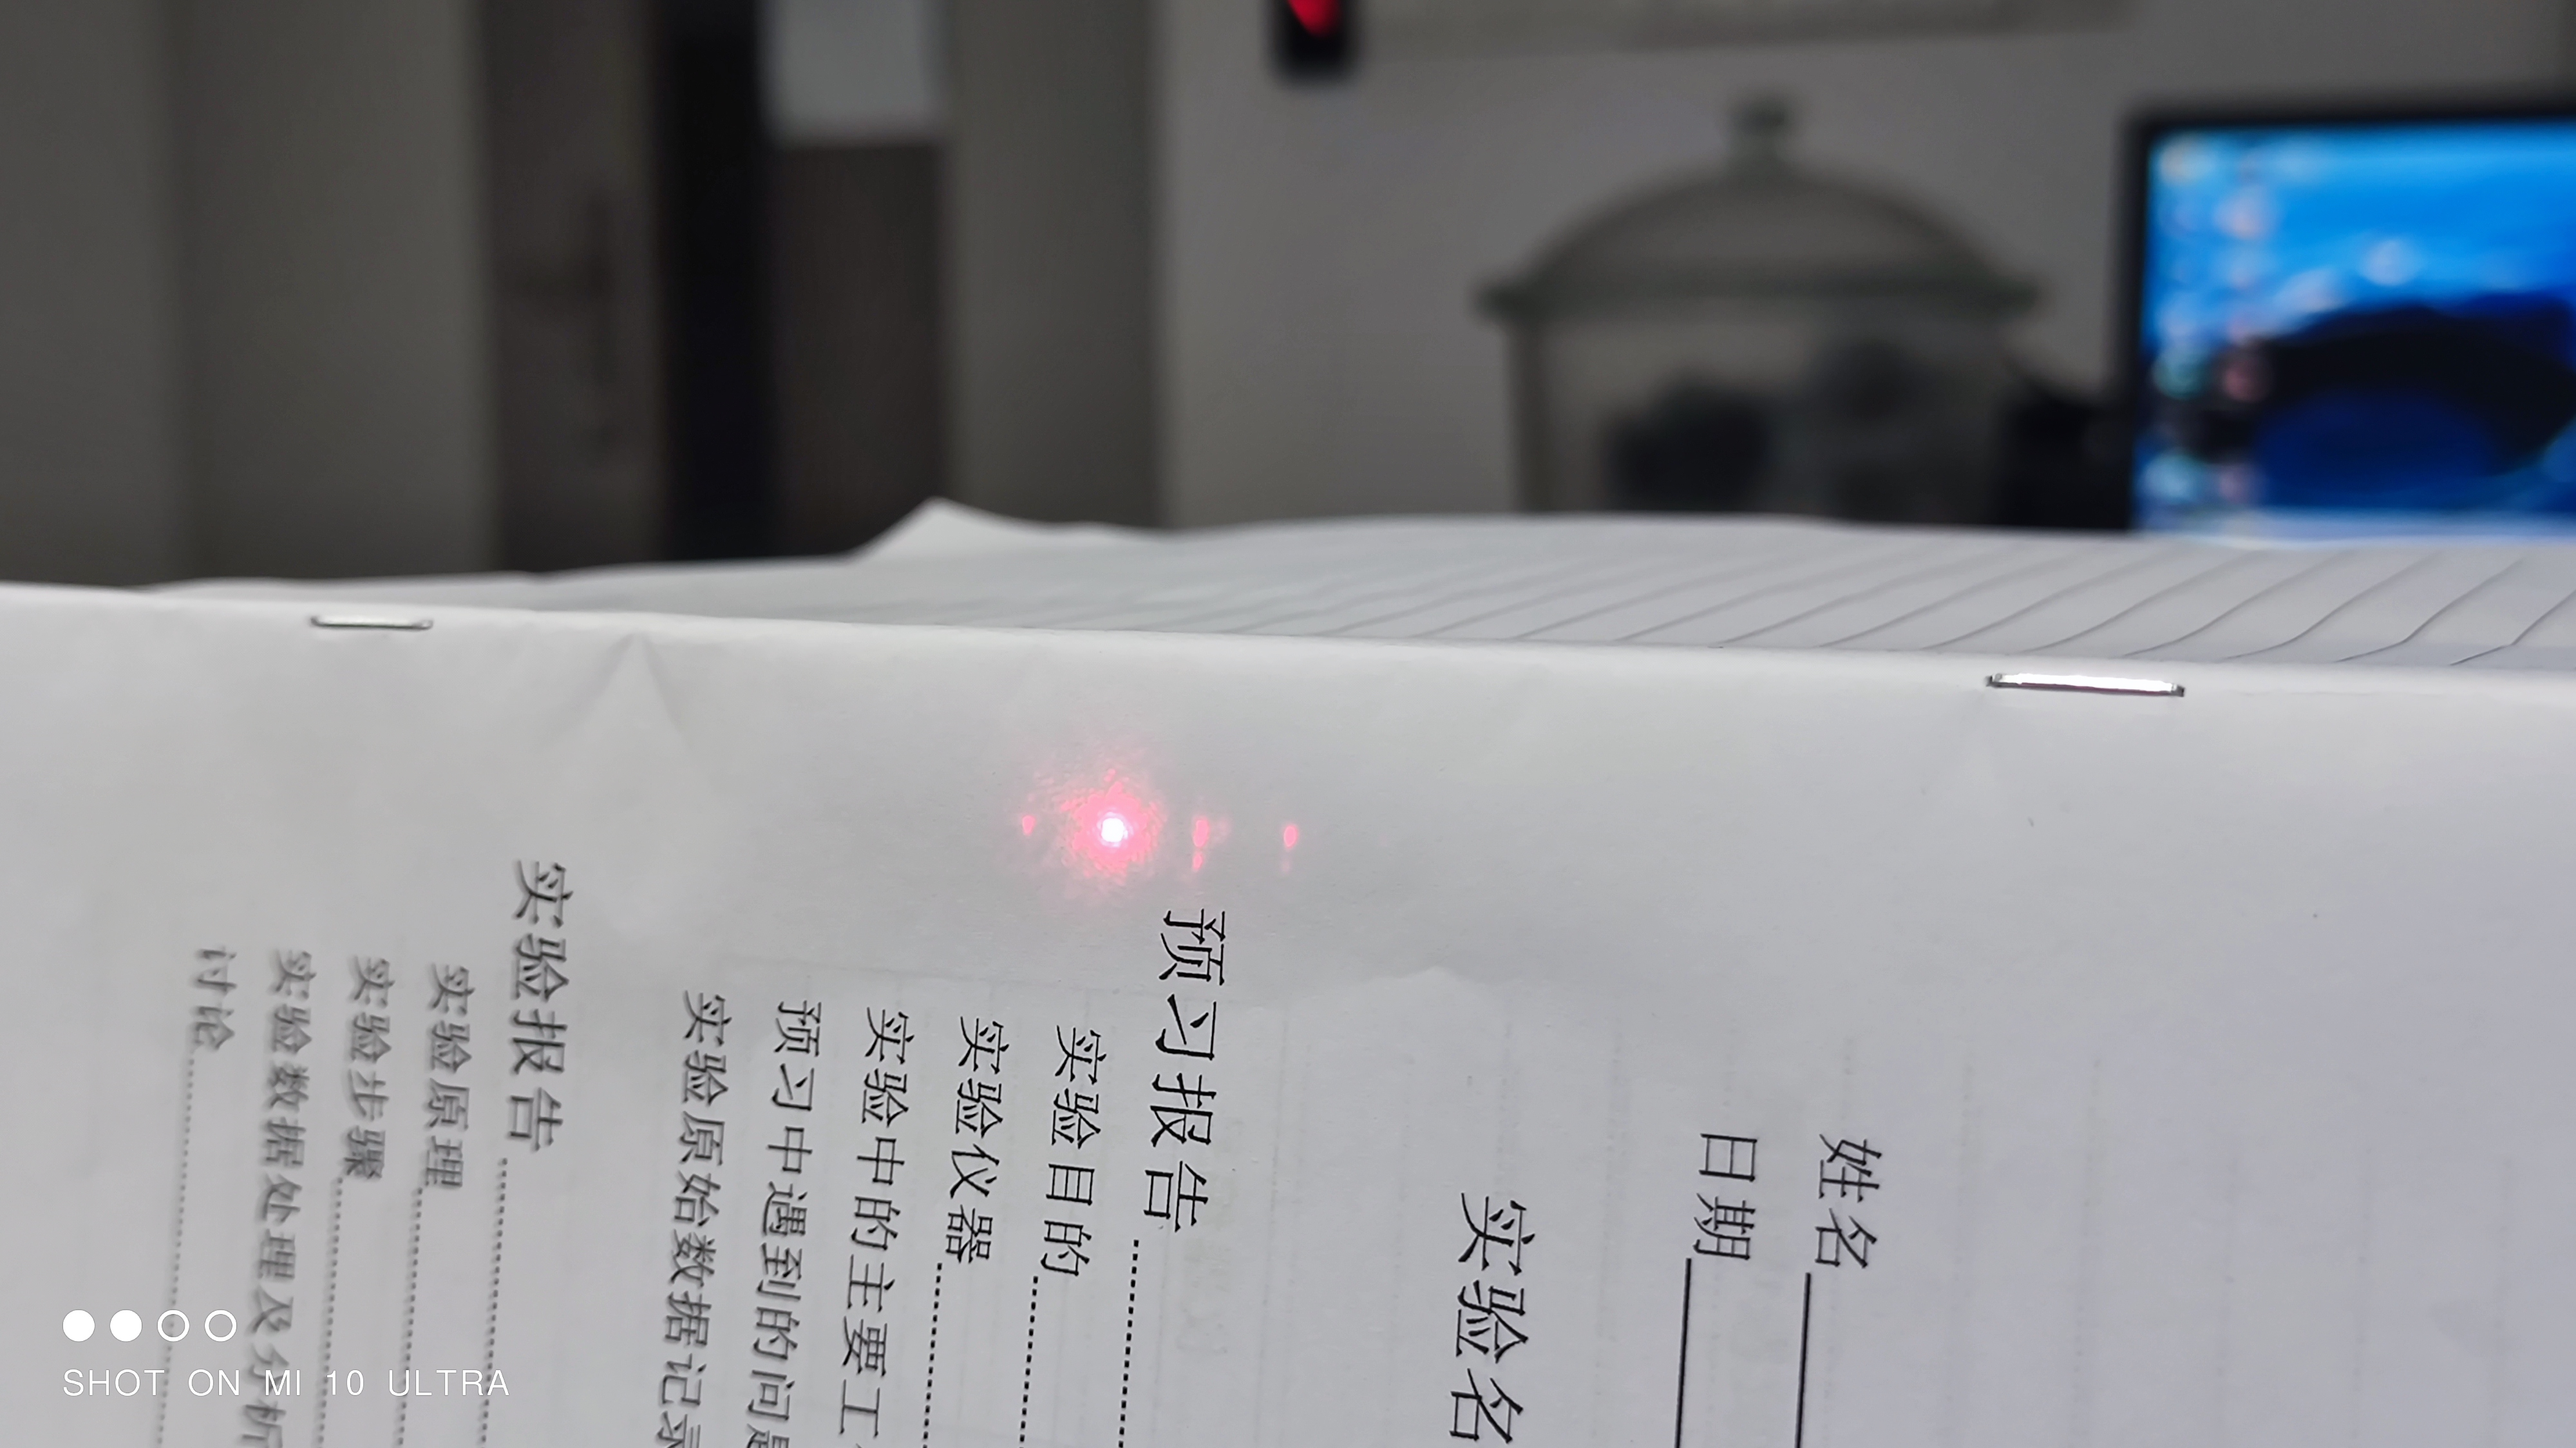
\includegraphics[scale=0.1]{pics/sp02.jpg}
    \end{figure}

    \begin{figure}[hp]
        \centering
        \caption{在示波器上确认 0 级光的位置}
        \subfloat[在介质中附加声波前]{
            \begin{minipage}{18em}
                \centering
                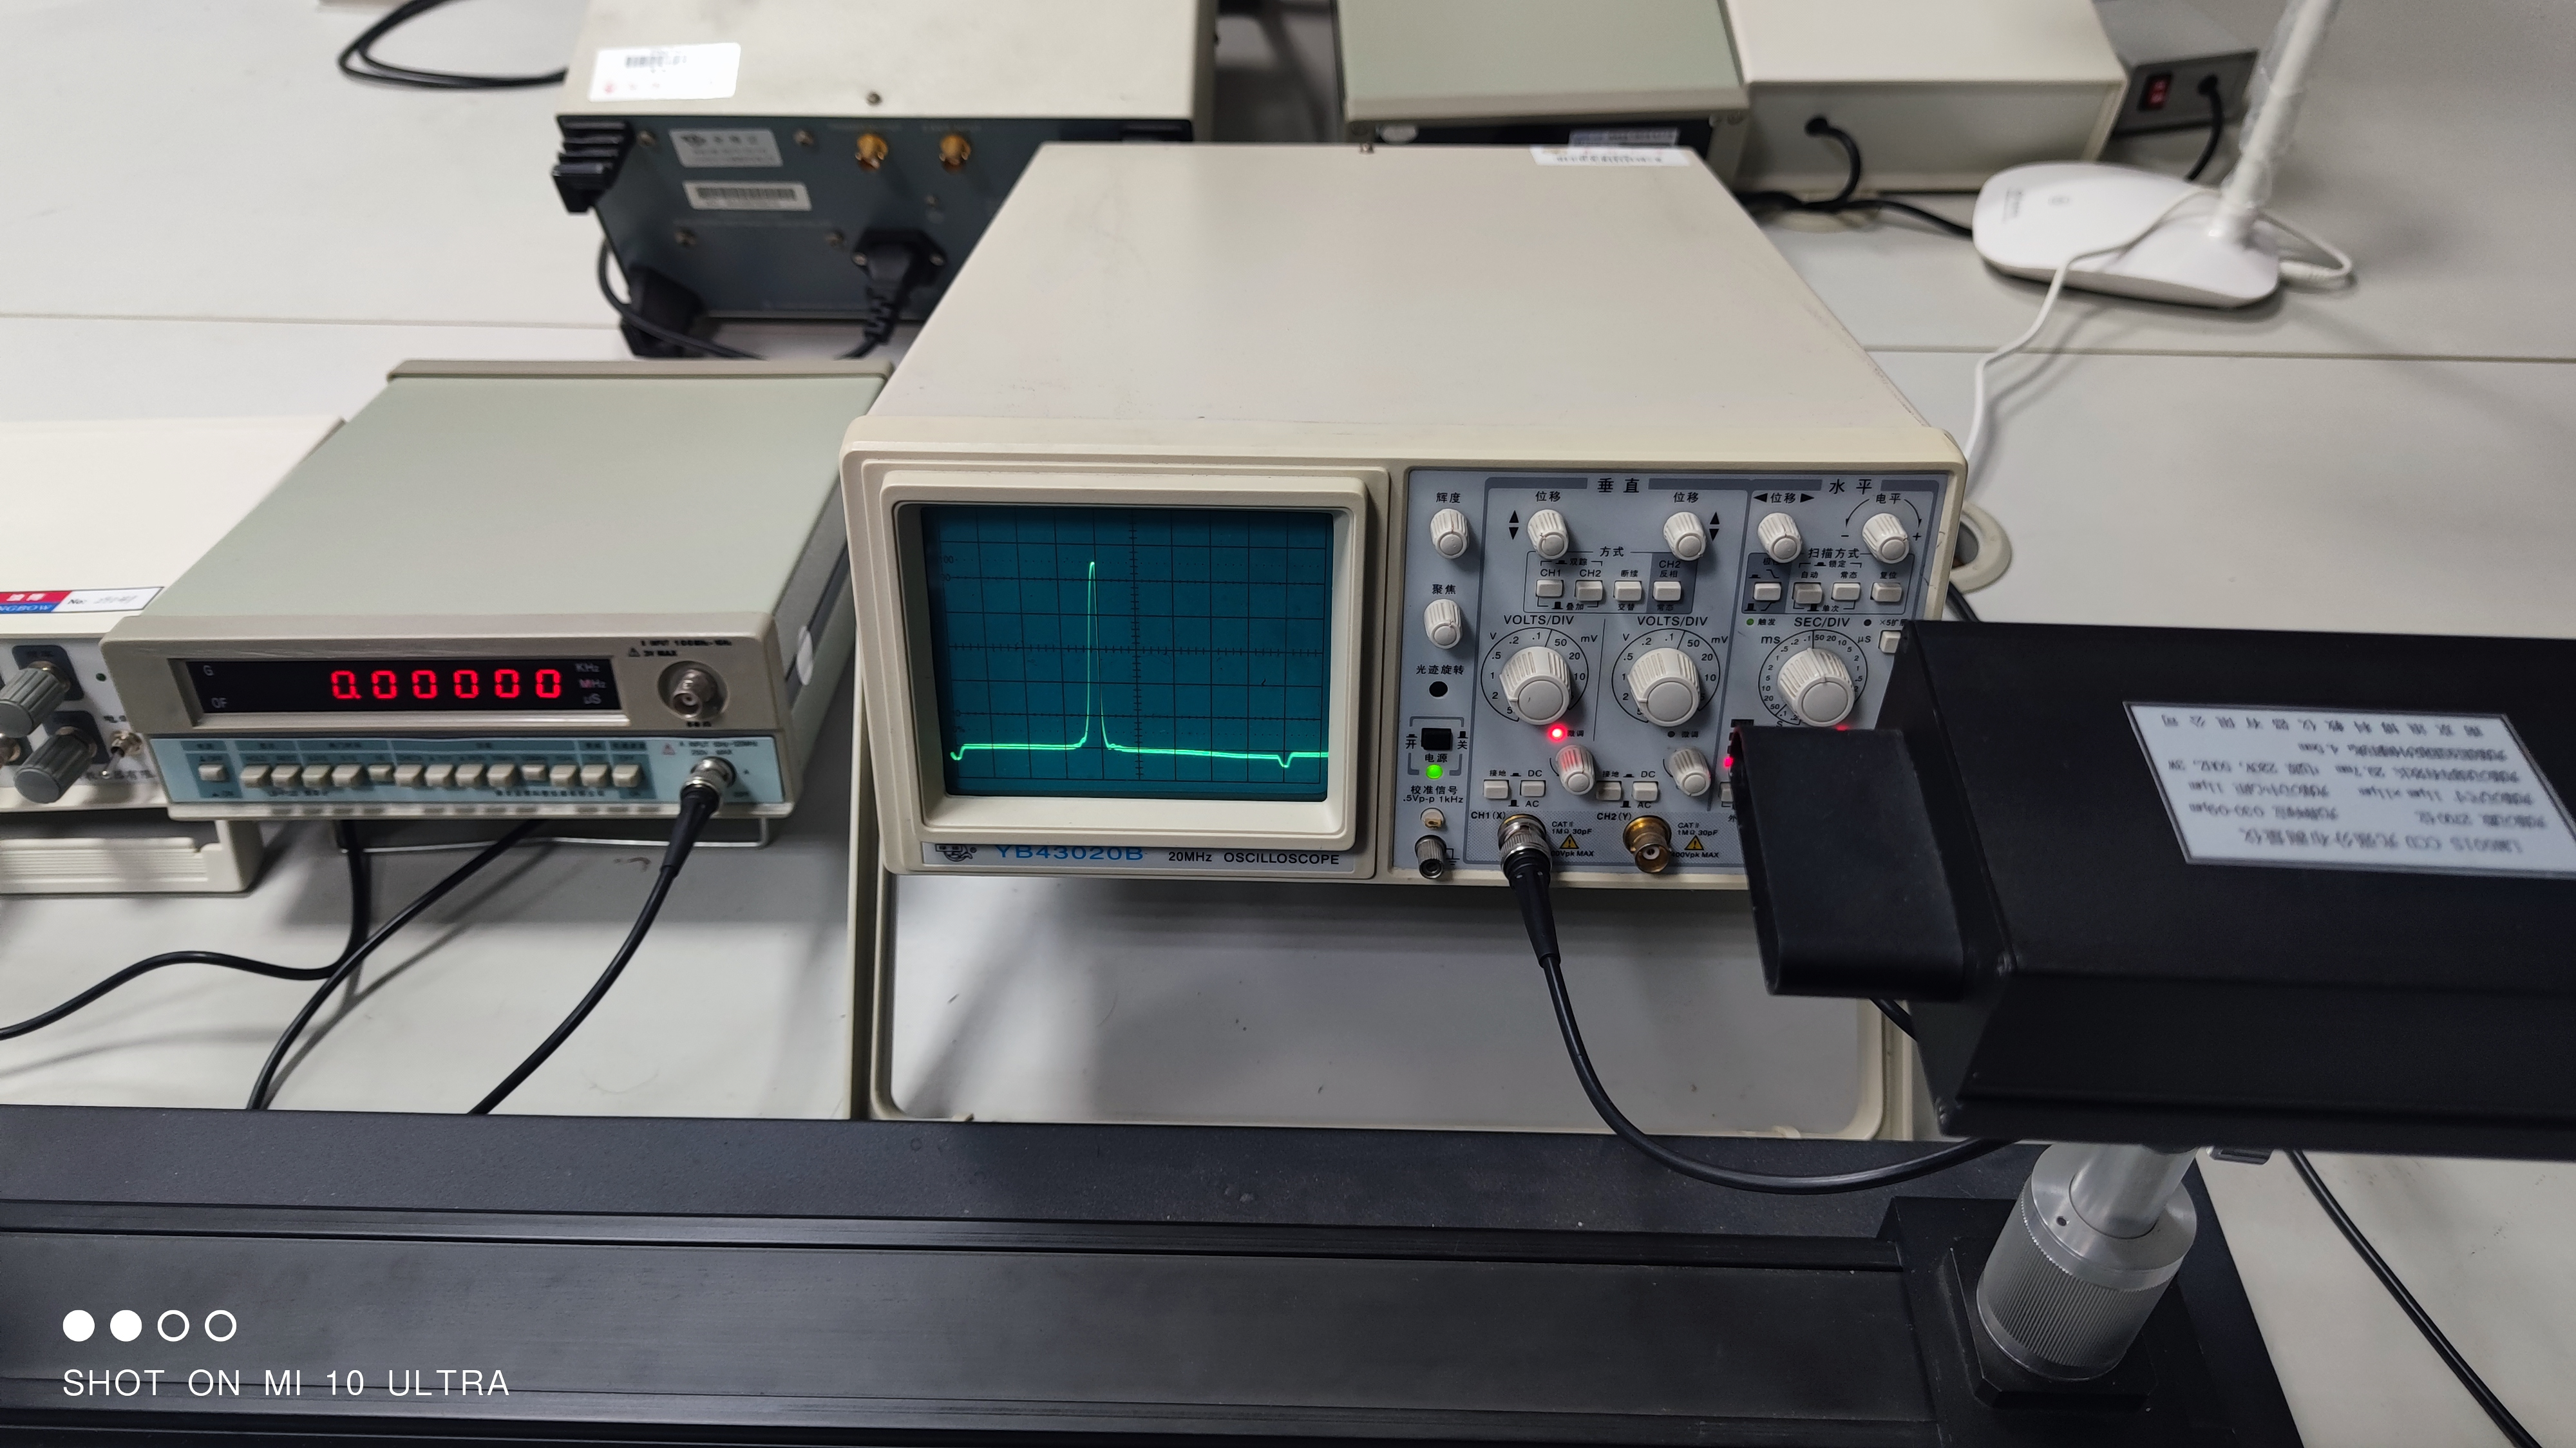
\includegraphics[scale=0.05]{pics/sp04-2.jpg}
            \end{minipage}
        }
        \subfloat[在介质中附加声波后]{
            \begin{minipage}{18em}
                \centering
                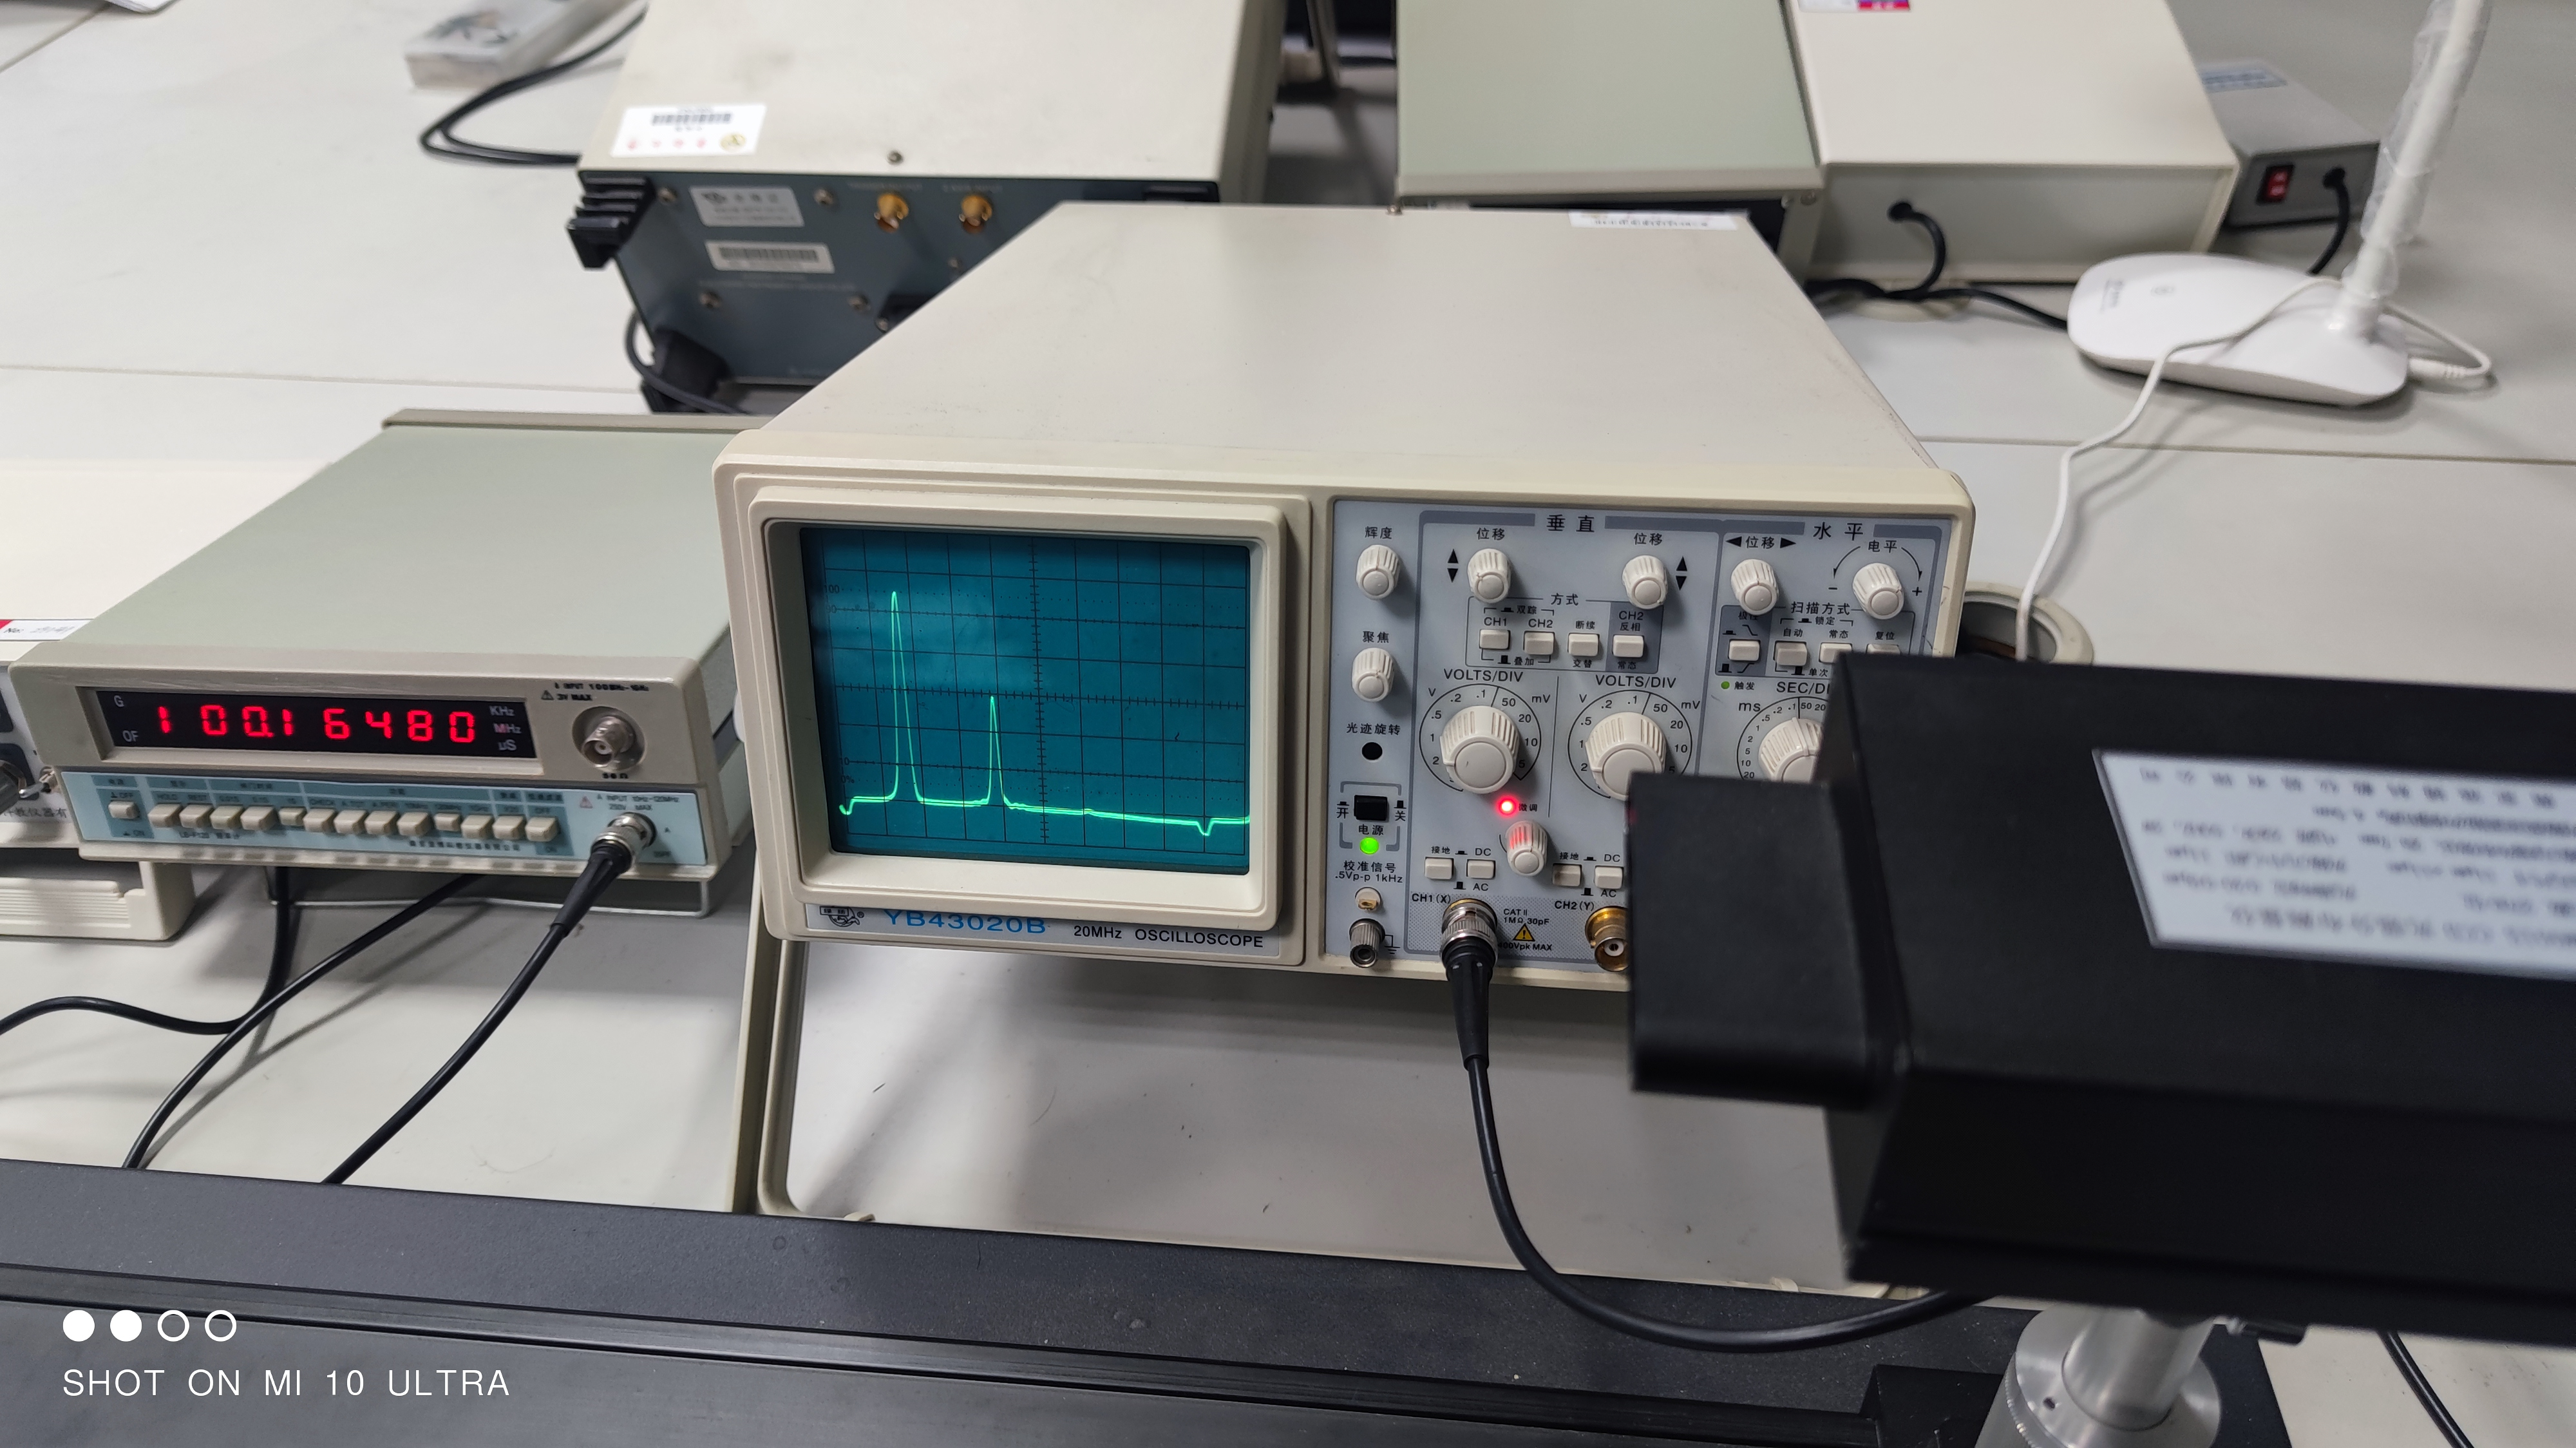
\includegraphics[scale=0.05]{pics/sp04-1.jpg}
            \end{minipage}
        }
    \end{figure}
\end{document}